\documentclass[12pt, a4paper]{article}
\usepackage[utf8]{inputenc}
\usepackage{footnote}
\usepackage{hyperref}
\usepackage{fullpage}
\usepackage{amsmath}
\usepackage{pgfplots}
\usepackage{pgfplotstable}
\pgfplotsset{compat=1.8}
\usepackage{cleveref}
\usepackage{graphicx}

\begin{document}
	\section{Vocabulary Statistics}
	\begin{itemize}
		\item latent variables (in statistics) are not observed, but rather inferred though other variables, that are observed
		\item observables (in statistics) are observed variables or factors of a dataset
		 \item generative model  in statistical classification including machine learning is not consistently defined, but wikipedia says "a generative model is a model of the conditional probability of the observable X given a target Y" $P(X|Y=y)$\footnote{\url{https://en.wikipedia.org/wiki/Generative_model}}
		 \item discriminative models are (following wikipedia) "are models of the conditional probability of the target Y, given observation x $P(Y|X=x)$"
		 \item unit Gaussian is the simplest gaussian distribution with unit variance and the integral equals to one
		 \item diagonal Gaussian ... from stackexchange.. special case where the only entries are on the diagonal.. an ellisoid in 3D...most of the mass concentrated near the center
		 \item mean - and log-variance
		 \item ELBO (evicence lower bound) ...only for VAE's??? dunno pls check
		 \item frequentist probability - repeatable event which results, if repeated enough times, leads to dirstribution of p; uncertainty related to the rate at which events occur
		 \item Bayesian probability - outcome not repeatable, but qualitatively described; qualitative level of uncertainty
	\end{itemize}
	\section{Vocabulary Python}
		\begin{itemize}
			\item super- inherit smth from one class to another
			\item keras.layers.Flatten - 
			\item reduce\_sum
			\item gradienttape
		\end{itemize}
	\section{Convolution Neural Network \\ 
			(tensorflow.org/tutorials/generative/cvae)}
		\subsection{Main Network Ideas}
	The generative and interference network are wired up with the Keras Model Sequential. \textbf{tf.keras.Sequential} is used for small networks. In this example 2 Convnets are bulid for the generative and interference network. The generative model takes a latent encoding as input, and outputs the parameters for a conditional distribution of the observation (x) $\rightarrow p(x|z)$. Additionally, a unit Gaussian prior $p(z)$ is used for the latent variable (z). The inference network defines an approximate posterior distribution $q(z|x)$. It takes as input an observation and outputs a set of parameters for the conditional distribution of the latent representation. q is defined as a diagonal Gaussian. The output is then the mean and log-variance of a factorized Gaussian. A reparameterization trick is used during optimization: durig optimization samples are taken from $q(z|x)$ by first sampling from a unit Gaussian, then multiplying by the standard deviation and adding the mean. "This ensures the gradients can pass through the sample to the inference network parameters."
	The inference network comprises two convolutional layers followed by a fully connected layer. The generative network mirrors this architecture by using a fully connected layer followed by three convolution transpose layers. \textbf{WHY?} it is common practice to avoid using batch normalization when training VAE's, since the additional stochasticity due to using mini-batches may aggravate instability on top of the stochastisity from sampling.
	\subsection{Loss function and optimizer}
	Maximizing the evidence lower bound (ELBO) on the marginal log-likelihood is typical to VAE:\\
	 $logp(x)\geq ELBO = E_{q(z|x)} \left[log\frac{p(x,z)}{q(z|x)}\right]$\\
	In practice, the single sample Monte Carlo estimate of this expectation is optimized:\\
	 $logp(x|z)+logp(z)-log(z|x)$, where z is samples from $q(z|x)$
	\subsection{Stopping here}
		The proposed CVAE did not work on my system eccept for the running in the juypiter notebook. As I am not using a variational autoencoder, this ection stops here. Working with tensorflow was first experienced here, so this experience is taken further.
	\section{Convolutional Autoencoder Sandia 2019}
	\subsection{Initial condition satisfaction}
	\section{Deep Learning from Ian Goodfellow et al.}
	\subsection{Statistics and Information Theory}
	\subsubsection{Mixture Distributions}
	A in machinelearning widely used term the latent variable is strongly based on mixture distributions. For a mixture of distributions a multinoulli distribution is utilized. A multinoulli distribution is a vecorized distribution over a single discrete variable with k states. Mixtures of distributions can be written as:
	$P(x)=\sum_{i} P(c=i)P(x|c=i)$.
	Where P(c) is a multinoulli distribution. Mixture distributions combine different distributions enhancing a richer model. In the example above c would be the latent variable.
	\subsubsection{Useful functions}
	Logistic sigmoid: $\sigma(x)=\frac{1}{1+exp(x)}$
	\subsection{5 Machine Learning Basics}
	Basic concepts of machine learning include accuracy and error-rate.	With accuracy the proportion of examples for which the model produces the correct is meant. The error-rate refers to the proportion of examples for which the model produces an incorrect output. The error-rate takes often a value between 0 and 1, where 0 means no loss and vice versa. The performance of a model is usually perfomred on a test set, which differs from the train set. Performance measure can be quiete individual for different tasks.\\
	Other concepts are Overfitting, Underfitting and the Capacity. Underfitting appears, when the error value on the training set is not sufficiently small enough. Overfitting on the other hand describes the discrepany between the error value on the test and the training set. A model is overfit, when the error value on the test set exceeds the error value on the training set.\\
	A model needs to perform well on unseen data, which brings rise to the generalization error. To control the generalization error, a few assumptions are made for the test and training data. The i.i.d. assumptions : First examples in each dataset are independend. Second train-set and test-set are identically distributed. Meaning, they have the same underlying distribution. \\
	The capacity of a model refers to its ability to fit a wide variety of functions (very informal discription). When overfitting, the models capacity includes functions, that do only fit the train set well, but not the test set. When underfitting the capacity of the model is to limited to fit the complexity of the train set. The family of functions a model can choose from to reduce a training objective is called its representational capacity. Effective capacity includes the imperfections of the optimization algorithm. methodds to control the capacity of the model and by that over and underfitting, is by altering the hypothesis space of the model (set of functions a model can choose).
	\subsection{Regularization}
	Another way to influence the models capcity in order to reach the optimal capacity is by choosing panilizing factors. Regularization is any modification we make to a learning algorithm, that is intended to reduce its generalization error, but not its training error.\footnote{Deep Learning, Ian Goodfellow, p.117}
	\subsubsection{Hyperparameters and validation Sets}
	Hyperparameters, introduced to control the algorithms behavior are not learned. If so, the model would tend to overfit too easily. An example of a capacity hyperparameter would be the maximum polynominal degree in an regression algorithm. The concept of validation sets is indroduced here. The training data consists of a test set and a training set, whereas the training set is subdivided again into a training and a validation set. The test set is not used to make any choice about about the model. It is only used to etimate the overall generalization error after all hyperparameters are set. Most of the time the training set is subdivided into training and validation set by means of a cut into disjoint subsets of size 0.8 and 0.2. The training is used to train the models hyperparameters, the validation set is used to estimate the generalization error during/after training and to "guide" the selection of hyperparameters accordingly. The generalization error of the validation set will underestimate the overall generalization error.
\section{Linear Autoencoder compared to POD v1}
A first working model of a linear autoencoder is proposed and evaluated on the density over space in time of the BGK equation. The same matrix as in POD is used as input data for the autoencoder:
		\[S = \begin{bmatrix}
	f(\xi_1,t_1,x_1)&\cdots &f(\xi_n,t_1,x_1) \\
	f(\xi_1,t_1,x_2)&\cdots &f(\xi_n,t_1,x_2) \\
	f(\xi_1,t_1,x_n)&\cdots &f(\xi_n,t_1,x_n)\\
	f(\xi_1,t_2,x_1)&\cdots &f(\xi_n,t_2,x_1)\\
	\vdots & \ddots & \vdots\\
	f(\xi_1,t_n,x_n)&\cdots &f(\xi_n,t_n,x_n)
	\end{bmatrix}\]
During training every 1000 epochs a sample against its prediction was printed in order to link the value of the L1-Loss to a prediction. Using this method a first verification of the model was achieved. Continuing the search for any possible shortage of the models performance, that this method could not cover, eg. samples lying between every 1000 sample, that the model was not able to reconstruct correctly, a second verification process is conducted. 
\begin{figure}[htb!]
	\centering
	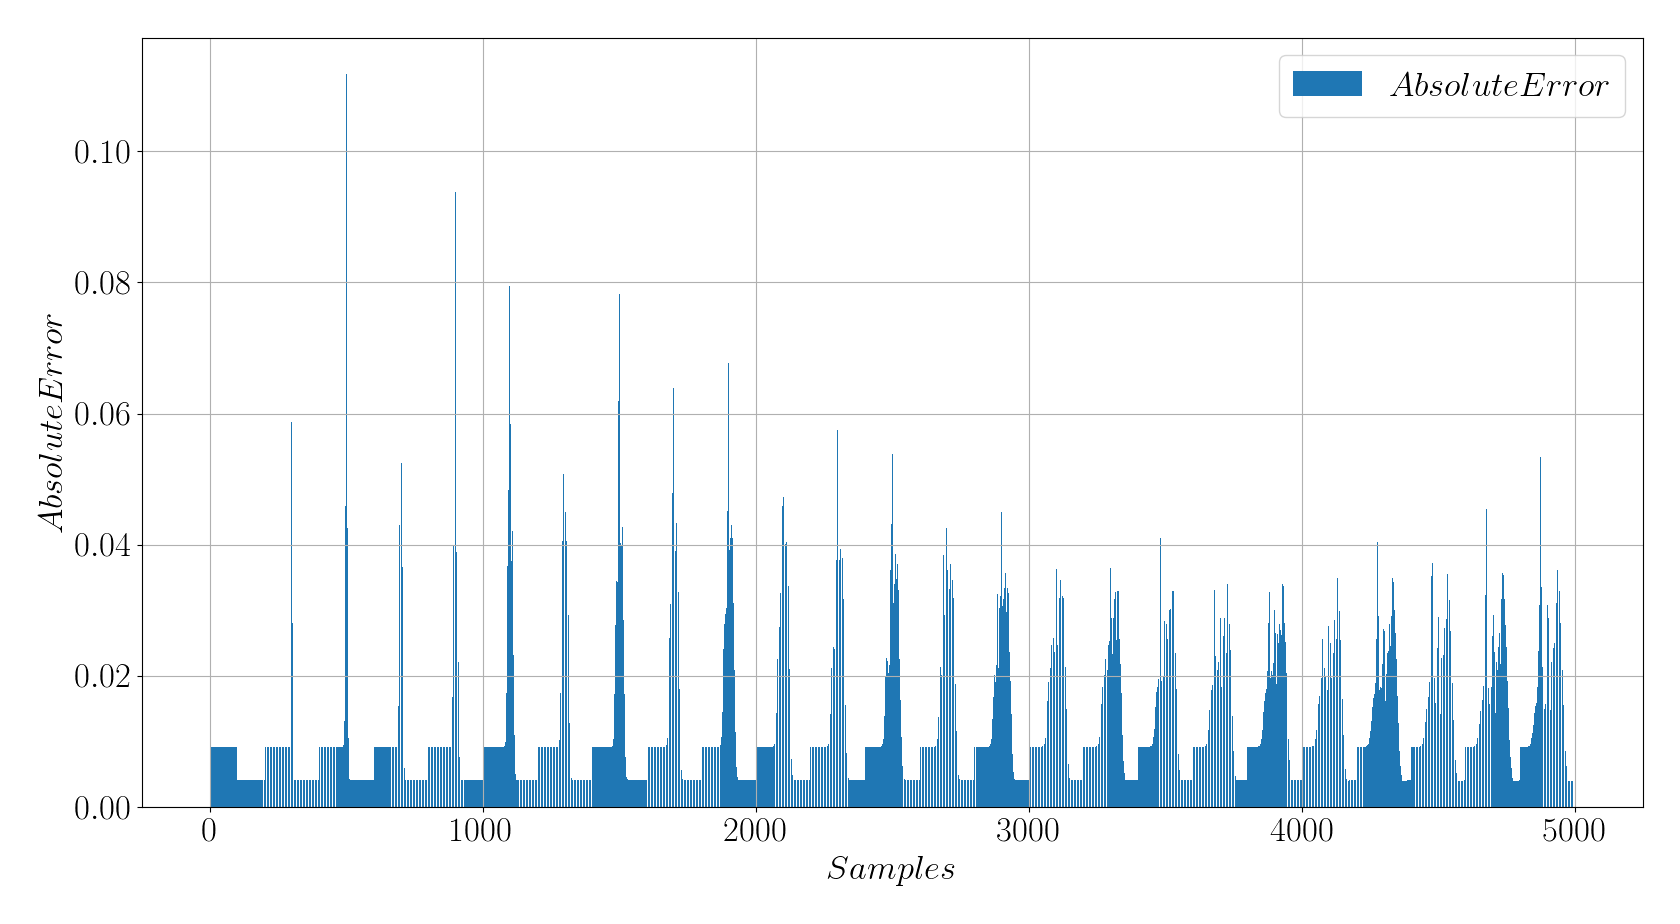
\includegraphics[width=.8\textwidth]{Error_samples_v1_1.png}
	\caption{Error of each sample}
	\label{Fig:error_sample}
\end{figure}
Inference is conducted after training using the same, but not shuffled input data. \Cref{Fig: error_sample} shows the error of every sample from the inference run. The largest mistake can be observed in sample 500. 
\begin{figure}[htb!]
	\centering
	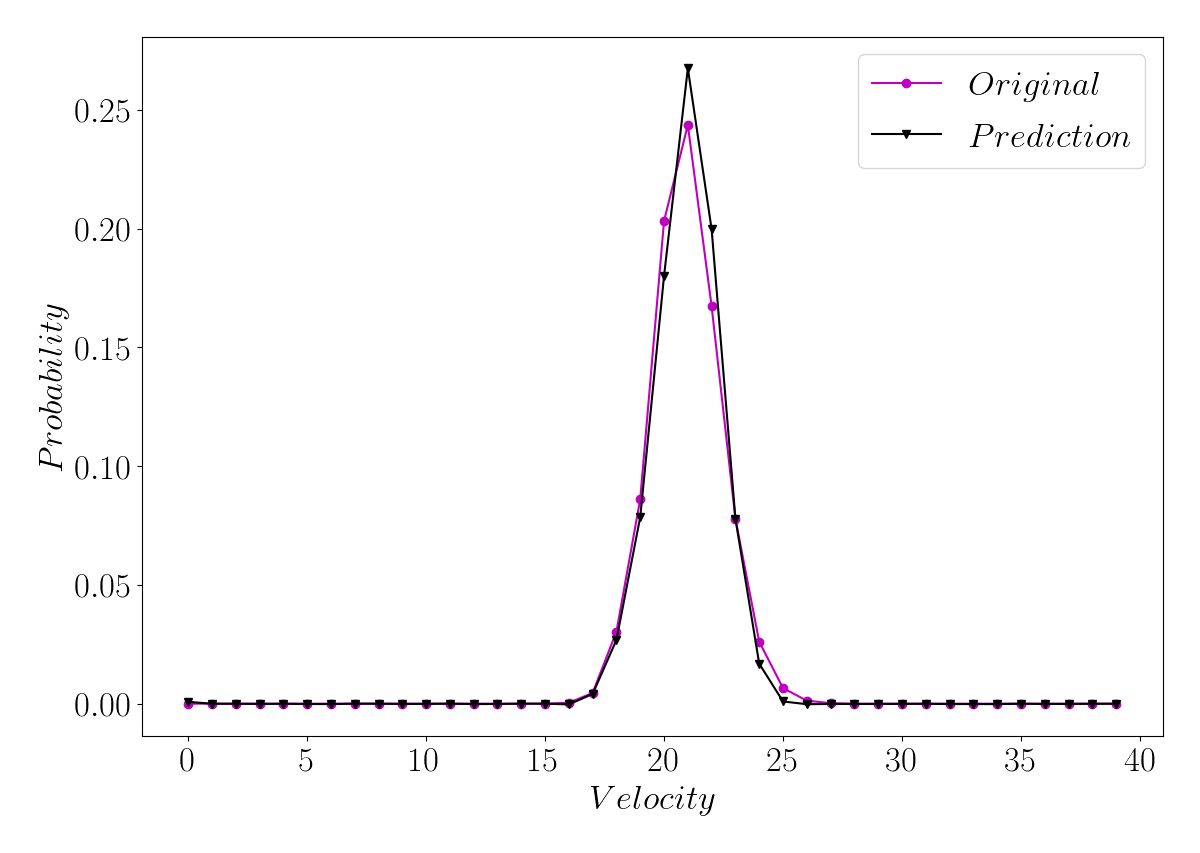
\includegraphics[width=.49\textwidth]{Sample500_v1_1.png}
	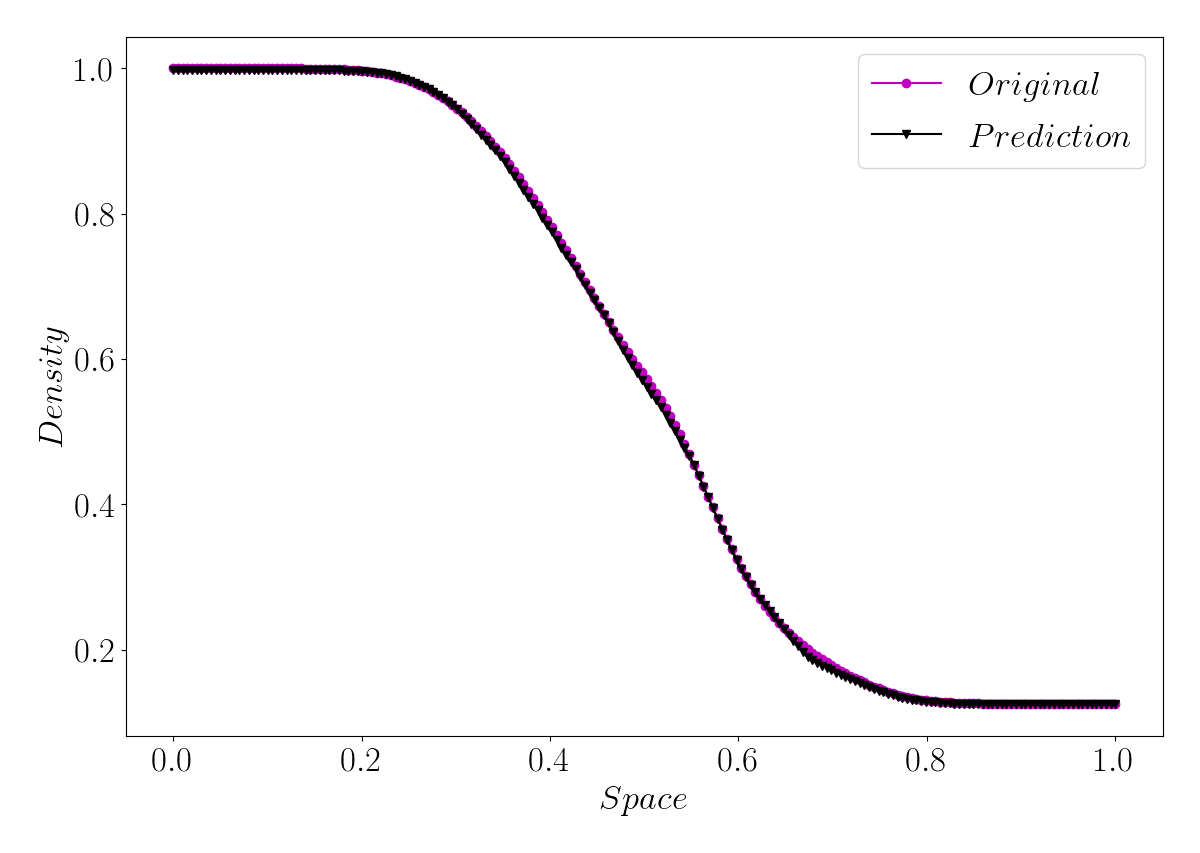
\includegraphics[width=.49\textwidth]{Density_last_v1_1.png}
	\caption{Error of each sample}
	\label{Fig:Errormore}
\end{figure}
Absolute Error for density is 0.59!!!!
\end{document}